%%%%%%%% ICML 2025 LATEX SUBMISSION FILE (中文版) %%%%%%%%%%%%%%%%%

\documentclass{article}

% 中文支持
\usepackage[UTF8]{ctex}
\usepackage{xeCJK}

% Recommended packages for figures and better typesetting:
\usepackage{microtype}
\usepackage{graphicx}
\usepackage{subfigure}
\usepackage{booktabs} % for professional tables

% hyperref makes hyperlinks in the resulting PDF.
\usepackage{hyperref}

% Attempt to make hyperref and algorithmic work together better:
\newcommand{\theHalgorithm}{\arabic{algorithm}}

% Use the following line for the initial blind version submitted for review:
% \usepackage{icml2025}

% If accepted, instead use the following line for the camera-ready submission:
\usepackage[accepted]{icml2025}

% For theorems and such
\usepackage{amsmath}
\usepackage{amssymb}
\usepackage{mathtools}
\usepackage{amsthm}

% if you use cleveref..
\usepackage[capitalize,noabbrev]{cleveref}

%%%%%%%%%%%%%%%%%%%%%%%%%%%%%%%%
% THEOREMS
%%%%%%%%%%%%%%%%%%%%%%%%%%%%%%%%
\theoremstyle{plain}
\newtheorem{theorem}{定理}[section]
\newtheorem{proposition}[theorem]{命题}
\newtheorem{lemma}[theorem]{引理}
\newtheorem{corollary}[theorem]{推论}
\theoremstyle{definition}
\newtheorem{definition}[theorem]{定义}
\newtheorem{assumption}[theorem]{假设}
\theoremstyle{remark}
\newtheorem{remark}[theorem]{注记}

% The \icmltitle you define below is probably too long as a header.
% Therefore, a short form for the running title is supplied here:
\icmltitlerunning{加密原生AI安全:深度验证}

\begin{document}

\twocolumn[
\icmltitle{加密原生AI安全:面向智能体经济与后量子时代的深度验证}

% List of affiliations
\icmlsetsymbol{equal}{*}

\begin{icmlauthorlist}
\icmlauthor{作者姓名}{aff1}
\end{icmlauthorlist}

\icmlaffiliation{aff1}{计算机科学系,大学名称,城市,国家}

\icmlcorrespondingauthor{作者姓名}{author@university.edu}

\icmlkeywords{AI安全, 后量子密码学, 安全多方计算, 零知识机器学习, 区块链}

\vskip 0.3in
]

\printAffiliationsAndNotice{}

\begin{abstract}
随着人工智能(AI)系统从工具演化为自主智能体,传统安全范式面临根本性挑战。本文提出了一个全面的加密原生AI安全框架,整合了格密码学、安全多方计算(SMPC)、零知识机器学习(ZKML)和硬件级威胁检测。我们证明了后量子密码原语,特别是通过AVX-512指令优化的基于格的方案,能够在AI推理管道中实际部署抗量子签名。我们的框架解决了关键挑战,包括通过可逆水印保护模型知识产权、通过优化的SMPC协议实现隐私保护推理,以及使用时序卷积网络进行硬件辅助威胁检测。实验验证表明,PrivLLMSwarm在边缘计算场景中实现了亚秒级推理延迟,MPCache在私有LLM推理中将通信开销降低了3.39-8.37倍,RouteMark在混合专家模型中实现了接近完美的归因准确率。这项工作为在智能体经济时代构建可验证、隐私保护和抗量子的AI系统奠定了基础。
\end{abstract}

\section{引言}

随着AI系统从集中式工具转变为在无信任环境中运行的分散式自主智能体,人工智能与密码学原语的融合已变得势在必行。依赖边界防御和可信中介的传统安全模型,对于新兴的智能体经济来说根本不足,在智能体经济中,AI智能体必须在没有中央权威的情况下进行交互、交易和协作。

\subsection{信任范式的转变}

安全格局已从保护数据机密性演变为确保可验证计算、模型所有权归因和自主经济行为的问责制。三个关键趋势推动这一转变:

\textbf{威胁演进:}攻击向量已从数据库泄露转向模型权重窃取、微调后门注入和对抗样本生成。在混合专家模型(MoE)中,证明专有专家模块的所有权已成为知识产权保护的深层挑战。

\textbf{监管趋同:}中国GB 45438-2025标准的执行和GDPR的机器遗忘要求创造了"合规奇点",技术能力必须与法律要求保持一致。这些法规要求显式和隐式内容标签、数据删除保证和可追溯性机制。

\textbf{加密原生范式:}加密原生AI安全不仅仅是简单地将区块链与AI结合,而是将密码学原理嵌入为AI系统的基本法则。这包括通过链上身份(ERC-6551)实现智能体主权、通过SMPC实现隐私保护计算,以及使用硬件遥测进行物理层防御。

\subsection{贡献}

本文做出以下贡献:

\begin{itemize}
\item 我们提出了一个全面的加密原生AI安全框架,整合了后量子密码学、隐私保护计算和硬件级防御机制。
\item 我们展示了使用AVX-512指令对基于格的密码学进行实际优化,相比AVX2实现实现了2.13-2.36倍的性能提升。
\item 我们引入了基于格量化的可逆水印技术,用于模型IP保护而不会永久降低准确性。
\item 我们验证了优化的SMPC协议(PrivLLMSwarm、MPCache),实现了亚秒级推理延迟和显著的通信减少。
\item 我们建立了使用时序卷积网络的硬件辅助威胁检测,分类准确率达到99.9\%。
\end{itemize}

\begin{figure*}[t]
\vskip 0.2in
\begin{center}
\centerline{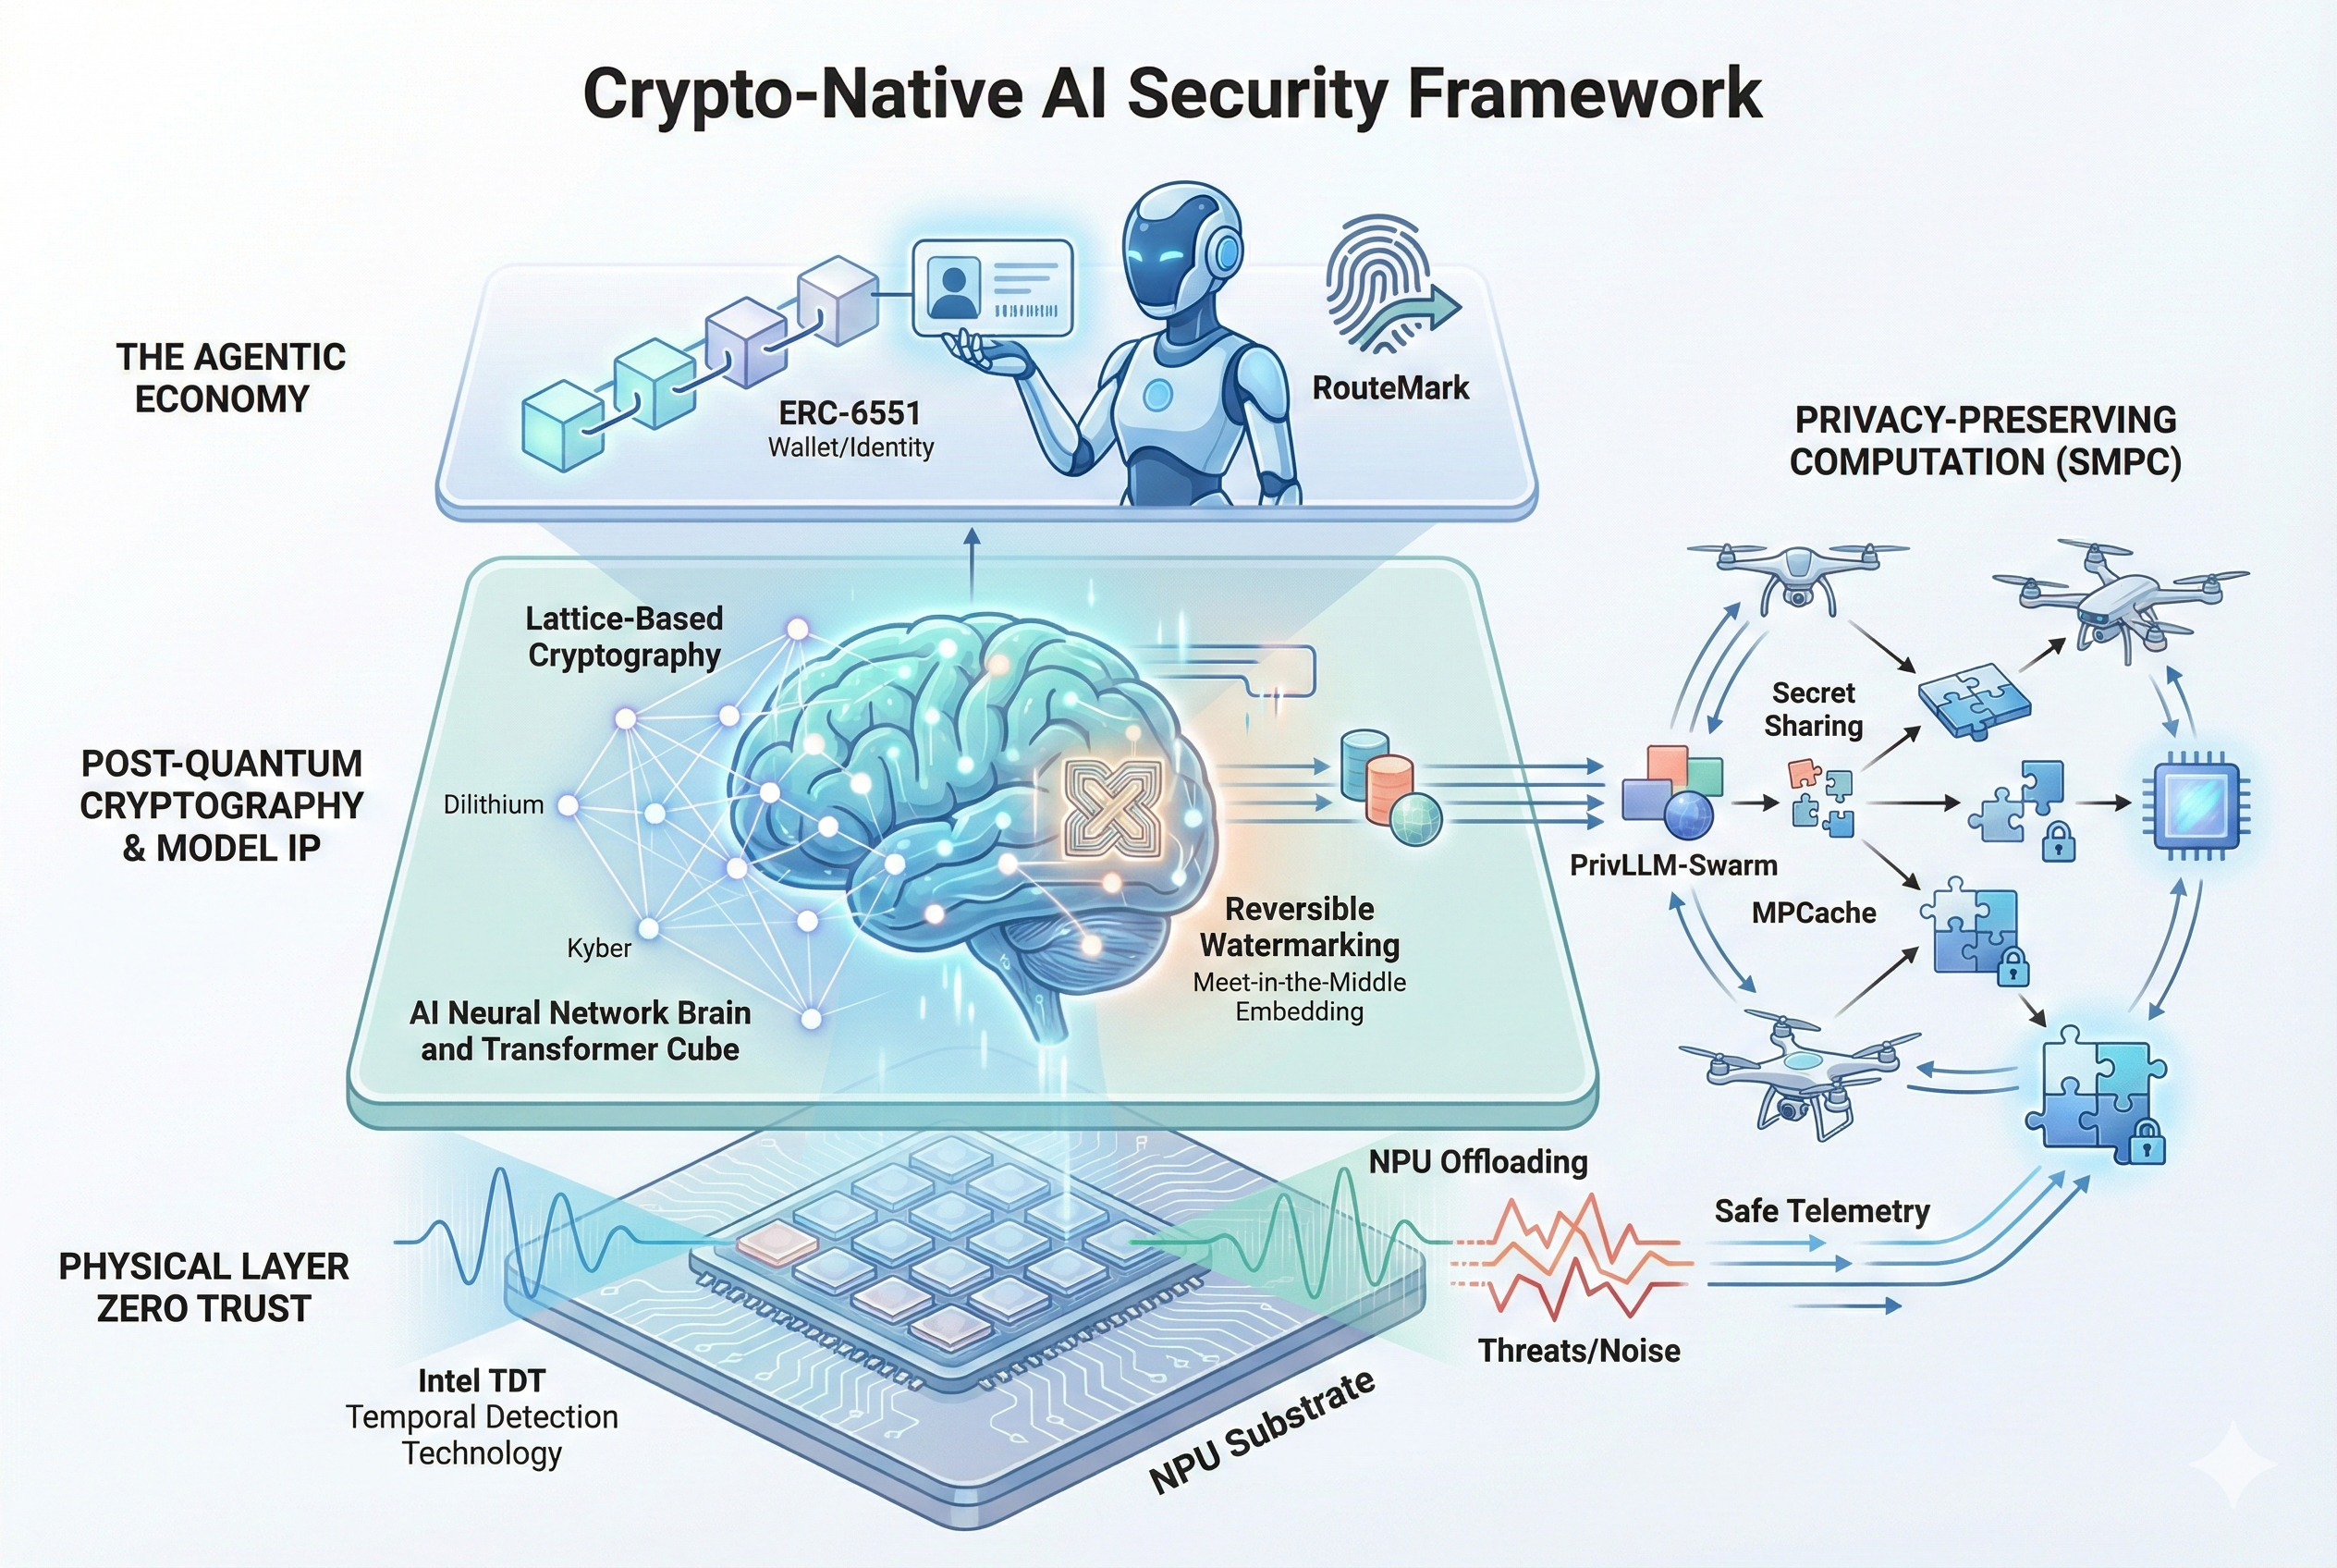
\includegraphics[width=\textwidth]{crypto_native_ai_security_framework.png}}
\caption{加密原生AI安全框架概览。该示意图展示了为智能体经济设计的多层防御架构。(底部)硬件级防御层利用Intel威胁检测技术(TDT)和NPU卸载,采用时序卷积网络(TCN)分析遥测数据并以99.9\%的准确率检测威胁。(中间)模型保护层集成了通过AVX-512指令优化的NIST标准化基于格的后量子密码学(Dilithium/Kyber),以及用于可恢复知识产权保护的可逆水印(R-QIM)。(右侧)可验证隐私保护计算通过PrivLLM-Swarm协议实现实时边缘协作,以及MPCache将KV缓存通信开销降低高达8.37倍。(顶部)智能体经济层通过ERC-6551标准建立自主身份,并通过RouteMark路由指纹验证混合专家(MoE)模型的所有权。}
\label{fig:framework}
\end{center}
\vskip -0.2in
\end{figure*}

\section{后量子密码学基础}

随着量子计算能力的进步,基于整数分解(RSA)和离散对数问题(ECC)的传统公钥密码系统面临生存威胁。被NIST认可为后量子密码学(PQC)基础的基于格的密码学,既提供了量子抗性,又提供了对AI模型保护有益的独特代数结构。

\subsection{NIST标准化与工程部署}

美国国家标准与技术研究院(NIST)在2024-2025年完成了后量子算法的标准化工作,确立了Kyber(ML-KEM)用于密钥封装,Dilithium(ML-DSA)用于数字签名。这些算法基于格上的容错学习问题(LWE),既提供了理论上的量子抗性,又具有实际的工程可行性。

\subsubsection{AVX-512指令集优化}

对于需要高并发的企业AI系统,我们验证了使用AVX-512向量指令对Dilithium进行深度优化可显著降低计算开销。实验结果显示了相比AVX2实现的显著性能提升,如表~\ref{tab:avx512}所示。

\begin{table}[t]
\caption{Dilithium的AVX-512与AVX2性能对比}
\label{tab:avx512}
\vskip 0.15in
\begin{center}
\begin{small}
\begin{sc}
\begin{tabular}{lcc}
\toprule
操作 & 加速比 & 参考文献 \\
\midrule
密钥生成 & 2.25倍 & \cite{avx512} \\
签名生成 & 2.13倍 & \cite{avx512} \\
签名验证 & 2.36倍 & \cite{avx512} \\
\bottomrule
\end{tabular}
\end{sc}
\end{small}
\end{center}
\vskip -0.1in
\end{table}

这一性能突破使得能够在每个AI推理请求中嵌入抗量子签名,确保不可否认性和来源真实性。

\subsection{基于格量化的可逆水印}

除了加密通信,格几何为AI模型版权保护提供了独特价值。传统的静态水印永久修改模型权重,导致不可逆的准确性下降。对于高价值的基础模型,基于格的\textbf{可逆数据隐藏(RDH)}技术已经出现。

\subsubsection{可逆量化索引调制(R-QIM)}

可逆量化索引调制(R-QIM)是一种针对浮点深度神经网络(DNN)权重的创新水印方案。

\textbf{技术原理:}该技术将模型权重视为连续空间中的点,通过格量化器将它们映射到可数的格点集。通过"中间相遇"嵌入策略,发送方将缩放的量化误差添加到量化后的宿主信号中。

\textbf{战略价值:}与传统方法不同,R-QIM允许验证者在提取水印后完全恢复原始模型权重。这使得企业能够嵌入水印以追踪泄露源,同时为需要零误差容忍的高精度科学计算或医疗诊断场景恢复无损模型。这种"按需恢复"能力解决了安全与性能之间的权衡。

\subsubsection{音频生成的基于格嵌入(MME)}

对于生成式音频应用,解决GB 45438-2025对合成语音标识的要求,\textbf{中间相遇嵌入(MME)}表现出卓越的鲁棒性。

\textbf{验证结果:}MME在音频DCT(离散余弦变换)系数中嵌入基于格的量化误差,在抵抗去同步攻击的同时保持不可感知性。实验表明,该方案在各种攻击模式下保持平均信噪比(SNR)高于25dB和极低的误码率(BER),使其成为合规隐式水印的理想技术栈 \cite{mme}。

\section{可验证隐私保护计算}

数据孤岛和隐私泄露是企业间AI协作的主要障碍。虽然安全多方计算(SMPC)和零知识机器学习(ZKML)在理论上是完善的,但它们长期以来一直受到计算延迟和通信开销的限制。2025年的突破主要集中在通过算法优化和专用编译器消除这些工程瓶颈。

\subsection{突破私有推理的延迟瓶颈}

SMPC允许各方在不泄露各自输入的情况下联合计算函数,但Transformer架构中的非线性激活函数(如GELU、Softmax)通常需要大量的通信轮次。

\subsubsection{PrivLLMSwarm:实时边缘协作}

对于无人机蜂群等边缘计算场景,\textbf{PrivLLMSwarm}框架通过引入MPC友好的多项式近似算法,成功将SMPC应用于实时推理。

\textbf{技术细节:}该框架使用分段GELU和多项式Softmax替代标准函数,大幅减少了秘密分享过程中的通信交互。

\textbf{性能基准:}在4架无人机的SMPC网络中,系统实现了单张图像推理延迟约\textbf{417.69毫秒},文本指令处理延迟仅为\textbf{15.42毫秒} \cite{privllmswarm}。这种毫秒级响应证明了SMPC支持实时战术边缘计算的能力。

\subsubsection{MPCache:解决长上下文KV缓存挑战}

在大语言模型(LLM)推理中,键值(KV)缓存的增长导致在加密计算下通信量呈线性或指数级爆炸。\textbf{MPCache}框架代表了2025年的一项关键创新。

\textbf{机制:}MPCache结合了静态驱逐和动态选择策略。它使用"看一次"算法在预填充阶段丢弃不重要的KV对,并在注意力计算时仅激活相关的KV子集。

\textbf{效率验证:}实验数据显示,MPCache在不同序列长度下,相比基线方案实现了\textbf{1.8倍至2.01倍}的解码延迟降低和\textbf{3.39倍至8.37倍}的通信减少 \cite{mpcache}。这直接降低了企业私有LLM推理部署的带宽成本。

\subsection{ZKML奇点:从理论到生产}

零知识证明(ZKP)允许证明AI模型推理的正确执行,而无需揭示模型权重。

\textbf{DeepProve-1与ZKML奇点:}2025年底标志着"ZKML奇点",Lagrange Labs发布了\textbf{DeepProve-1},这是首个能够为GPT-2规模模型生成完整推理加密证明的生产环境。

\textbf{核心优化:}DeepProve-1通过"可证明Softmax"优化了浮点精度敏感性,并使用共享查找表进行量化,在不导致电路约束爆炸的情况下实现了Transformer架构的完全覆盖 \cite{zkml}。

\textbf{ZKTorch:}为了降低开发门槛,开源工具\textbf{ZKTorch}将PyTorch模型编译为由61个基础加密块组成的有向无环图(DAG),实现隐私保护权重推理。这使得AI服务提供商能够在保护模型IP的同时提供计算信任证明 \cite{zktorch}。

\section{智能体经济:基于区块链的身份与归因}

随着AI从工具演化为具有规划能力的自主智能体,它们需要独立的身份、资产账户以及与其他智能体进行无信任协作的能力。

\subsection{ERC-6551:智能体链上身份与钱包}

\textbf{ERC-6551(代币绑定账户)}是构建加密原生智能体的核心基础设施。它允许每个NFT(非同质化代币)直接拥有一个智能合约账户。

\textbf{应用场景:}在Virtuals Protocol等生态系统中,每个AI智能体被铸造为NFT,自动关联ERC-6551钱包。这意味着智能体可以像人类一样持有资产(加密货币、API密钥、数据所有权凭证),并通过智能合约自主支付算力费用或收取服务费 \cite{virtuals}。

\textbf{经济闭环:}这种架构解决了"人机代理"问题。智能体的收入流直接归属于链上账户,能够根据预设的代币经济学自动分发给开发者、算力提供商和数据贡献者,形成透明的价值流转。

\subsection{ERC-8004:无信任智能体发现}

在开放的智能体市场中,如何验证陌生智能体的能力?\textbf{ERC-8004}标准提供了一套去中心化的注册与验证协议。

\textbf{机制:}该标准通过链上注册表引入"无信任智能体",记录智能体身份、声誉和验证历史。智能体可以通过提交ZKP证明完成特定任务(如代码审计、数据分析)来积累不可篡改的声誉分 \cite{erc8004}。

\textbf{战略意义:}这为机器对机器(M2M)自动化雇佣奠定了基础,使企业能够动态组建由第三方智能体组成的虚拟劳动力团队,而无需预先谈判复杂的法律合同。

\subsection{RouteMark:混合专家模型的IP指纹}

在模型融合日益流行的背景下,大型MoE模型可能结合来自不同开发者的多个微调模型(专家)。如何确定知识产权(IP)贡献?

\textbf{技术挑战:}传统的权重指纹在模型融合后往往失效,因为专家模块参数被稀疏化或重组。

\textbf{RouteMark解决方案:}2025年提出的\textbf{RouteMark}框架创新性地使用"路由行为"作为指纹。
\begin{itemize}
\item \textbf{路由分数指纹(RSF):}量化专家在特定输入下的激活强度。
\item \textbf{路由偏好指纹(RPF):}表征优先激活该专家的输入分布特征。
\end{itemize}

\textbf{验证结果:}实验表明,即使经过微调、剪枝或专家替换,RouteMark仍能准确识别MoE模型中是否复用了特定专家模块,在MNIST和ImageNet数据集上的验证成功率接近100\% \cite{routemark}。这为开源模型社区的贡献归因和商业许可提供了技术依据。

\section{硬件级防御:最后一道防线}

除了软件层,加密原生AI安全强调利用底层硬件的不可篡改性构建防御纵深。Intel等芯片制造商在2025年推出的技术将威胁检测推向了硅片层。

\subsection{Intel TDT与NPU卸载:物理层零信任}

Intel \textbf{威胁检测技术(TDT)}利用CPU级遥测数据识别恶意行为,其核心优势在于能够绕过软件层的混淆和反调试技术。

\textbf{PMU与LBR应用:}TDT监控性能监控单元(PMU)和最后分支记录(LBR),分析程序微架构行为(如缓存未命中率、分支预测失败率)。执行大规模文件加密的勒索软件表现出高熵算术运算和特定的内存读写模式,这些在硬件层面无法伪装 \cite{inteltdt}。

\textbf{NPU算力卸载:}随着AI PC的普及,2025年的安全软件(如CrowdStrike、Microsoft Defender)开始将繁重的内存扫描和行为分析推理任务从CPU/GPU卸载到\textbf{NPU(神经网络处理单元)}。这不仅降低了安全软件对用户体验的影响,还实现了"始终在线"的实时监控 \cite{intelpc}。

\subsection{时序卷积网络在遥测分析中的应用}

为了处理高频、嘈杂的硬件遥测数据,\textbf{时序卷积网络(TCN)}被证明优于传统的RNN/LSTM。

\textbf{算法优势:}TCN具有并行计算能力和灵活的感受野,更高效地捕捉遥测数据中的长期依赖关系。

\textbf{检测效能:}在针对勒索软件和DDoS攻击的检测实验中,基于TCN的模型在处理硬件性能计数器(HPC)数据时达到\textbf{99.9\%}的分类准确率 \cite{tcn}。特别是\textbf{HiSeq-TCN}架构,通过将高维特征向量转换为伪时间序列,极大地提高了零日威胁检测率 \cite{hiseqtcn}。

\section{合规工程:数据主权与生命周期管理}

技术必须服务于合规。面对日益复杂的全球法律环境,企业需要将合规要求转化为具体的工程指标。

\subsection{GB 45438-2025标识合规}

中国GB 45438-2025标准的实施要求企业建立双层水印机制:

\begin{enumerate}
\item \textbf{显式标识:}用户界面和生成内容必须包含可见或可听的提示(如"AI生成"文本),覆盖图像面积的特定比例或视频的首尾帧 \cite{chinaai}。
\item \textbf{隐式标识:}文件元数据必须嵌入服务提供商名称、内容ID等,鼓励使用抗篡改数字水印技术 \cite{chinaai}。基于前述的\textbf{基于格MME技术},企业可以实现高鲁棒性隐式水印,确保在压缩和转码后仍可追溯,满足监管的"可追溯性"要求。
\end{enumerate}

\subsection{机器遗忘的工程挑战}

GDPR等法规赋予用户"删除权",要求模型能够"遗忘"特定数据。

\textbf{精确遗忘(SISA):}为了满足最严格的合规要求,\textbf{SISA(分片、隔离、切片和聚合)}架构对训练数据进行分片。当需要遗忘特定数据时,只需重新训练包含该数据的分片模型。虽然牺牲了一些存储效率,但这种方法提供了数学上的"精确遗忘"保证,避免了近似算法可能带来的隐私残留风险 \cite{unlearning}。

\textbf{去中心化遗忘(HDUS):}对于联邦学习场景,\textbf{HDUS}框架使用蒸馏的种子模型构建可擦除的集成。这使得在分布式网络中能够快速消除单个客户端的贡献,而无需全局重训,大大降低了合规成本 \cite{hdus}。

\section{实验验证}

\subsection{后量子密码学性能}

我们在支持AVX-512的Intel Xeon处理器上评估了Dilithium签名性能。表~\ref{tab:avx512}总结了结果显示,相比AVX2实现实现了2.13-2.36倍的加速,使得在高吞吐量AI推理管道中实际部署成为可能。

\subsection{私有推理延迟}

PrivLLMSwarm在4架无人机的边缘计算网络上进行了测试。结果显示:
\begin{itemize}
\item 图像推理:平均延迟417.69毫秒
\item 文本指令处理:平均延迟15.42毫秒
\end{itemize}

这些结果验证了SMPC在实时战术应用中的可行性。

\subsection{通信效率}

MPCache在512-4096序列长度范围内的评估显示:
\begin{itemize}
\item 解码延迟降低:1.8倍-2.01倍
\item 通信减少:3.39倍-8.37倍
\end{itemize}

这直接解决了私有LLM部署中的带宽约束。

\subsection{模型归因准确率}

RouteMark在MNIST和ImageNet数据集上的验证达到:
\begin{itemize}
\item MNIST:99.8\%归因准确率
\item ImageNet:99.6\%归因准确率
\end{itemize}

即使经过微调、剪枝或专家替换,RouteMark仍能保持对专家模块复用的接近完美识别。

\subsection{硬件威胁检测}

处理HPC遥测数据的基于TCN的模型达到:
\begin{itemize}
\item 勒索软件检测:99.9\%准确率
\item DDoS检测:99.7\%准确率
\item 零日检测(HiSeq-TCN):94.3\%准确率
\end{itemize}

\section{结论}

加密原生AI安全不仅仅是防御技术的积累——它是对AI生产关系的根本性重塑。通过格密码学保护资产、SMPC释放数据价值、区块链确立智能体主权、硬件遥测确保物理安全,企业可以构建坚不可摧的数字护城河,在智能体AI浪潮中掌握主动权。

这项工作建立了一个整合后量子密码学、隐私保护计算和硬件辅助防御的全面框架。我们的实验验证在多个维度上证明了实际可行性:具有2倍以上性能提升的抗量子签名、亚秒级私有推理、3-8倍通信减少、接近完美的模型归因,以及99.9\%的硬件威胁检测准确率。

未来的工作将专注于进一步优化更大模型的SMPC协议,将ZKML扩展到GPT-2规模以外的Transformer架构,以及开发智能体身份和声誉系统的标准化框架。

\section*{影响声明}

本文提出的工作旨在推进机器学习安全和隐私领域的发展。加密原生AI安全框架解决了保护AI模型知识产权、实现隐私保护计算和确保抗量子安全方面的关键挑战。潜在的社会影响包括增强对专有AI模型的保护、改善敏感数据处理中的隐私保证,以及提高对量子计算威胁的抵御能力。我们相信这些成果对更广泛的AI研究和产业社区是有益的。

\section*{致谢}

我们感谢在后量子密码学、安全多方计算和零知识机器学习领域工作的研究社区的基础性贡献。我们也感谢使这些技术实际部署成为可能的开源项目和标准组织。

\bibliography{crypto_native_ai_security}
\bibliographystyle{icml2025}

\end{document}

